\begin{figure}
 \centering
    \begin{subfigure}[b]{0.5\textwidth}
        \centering
    	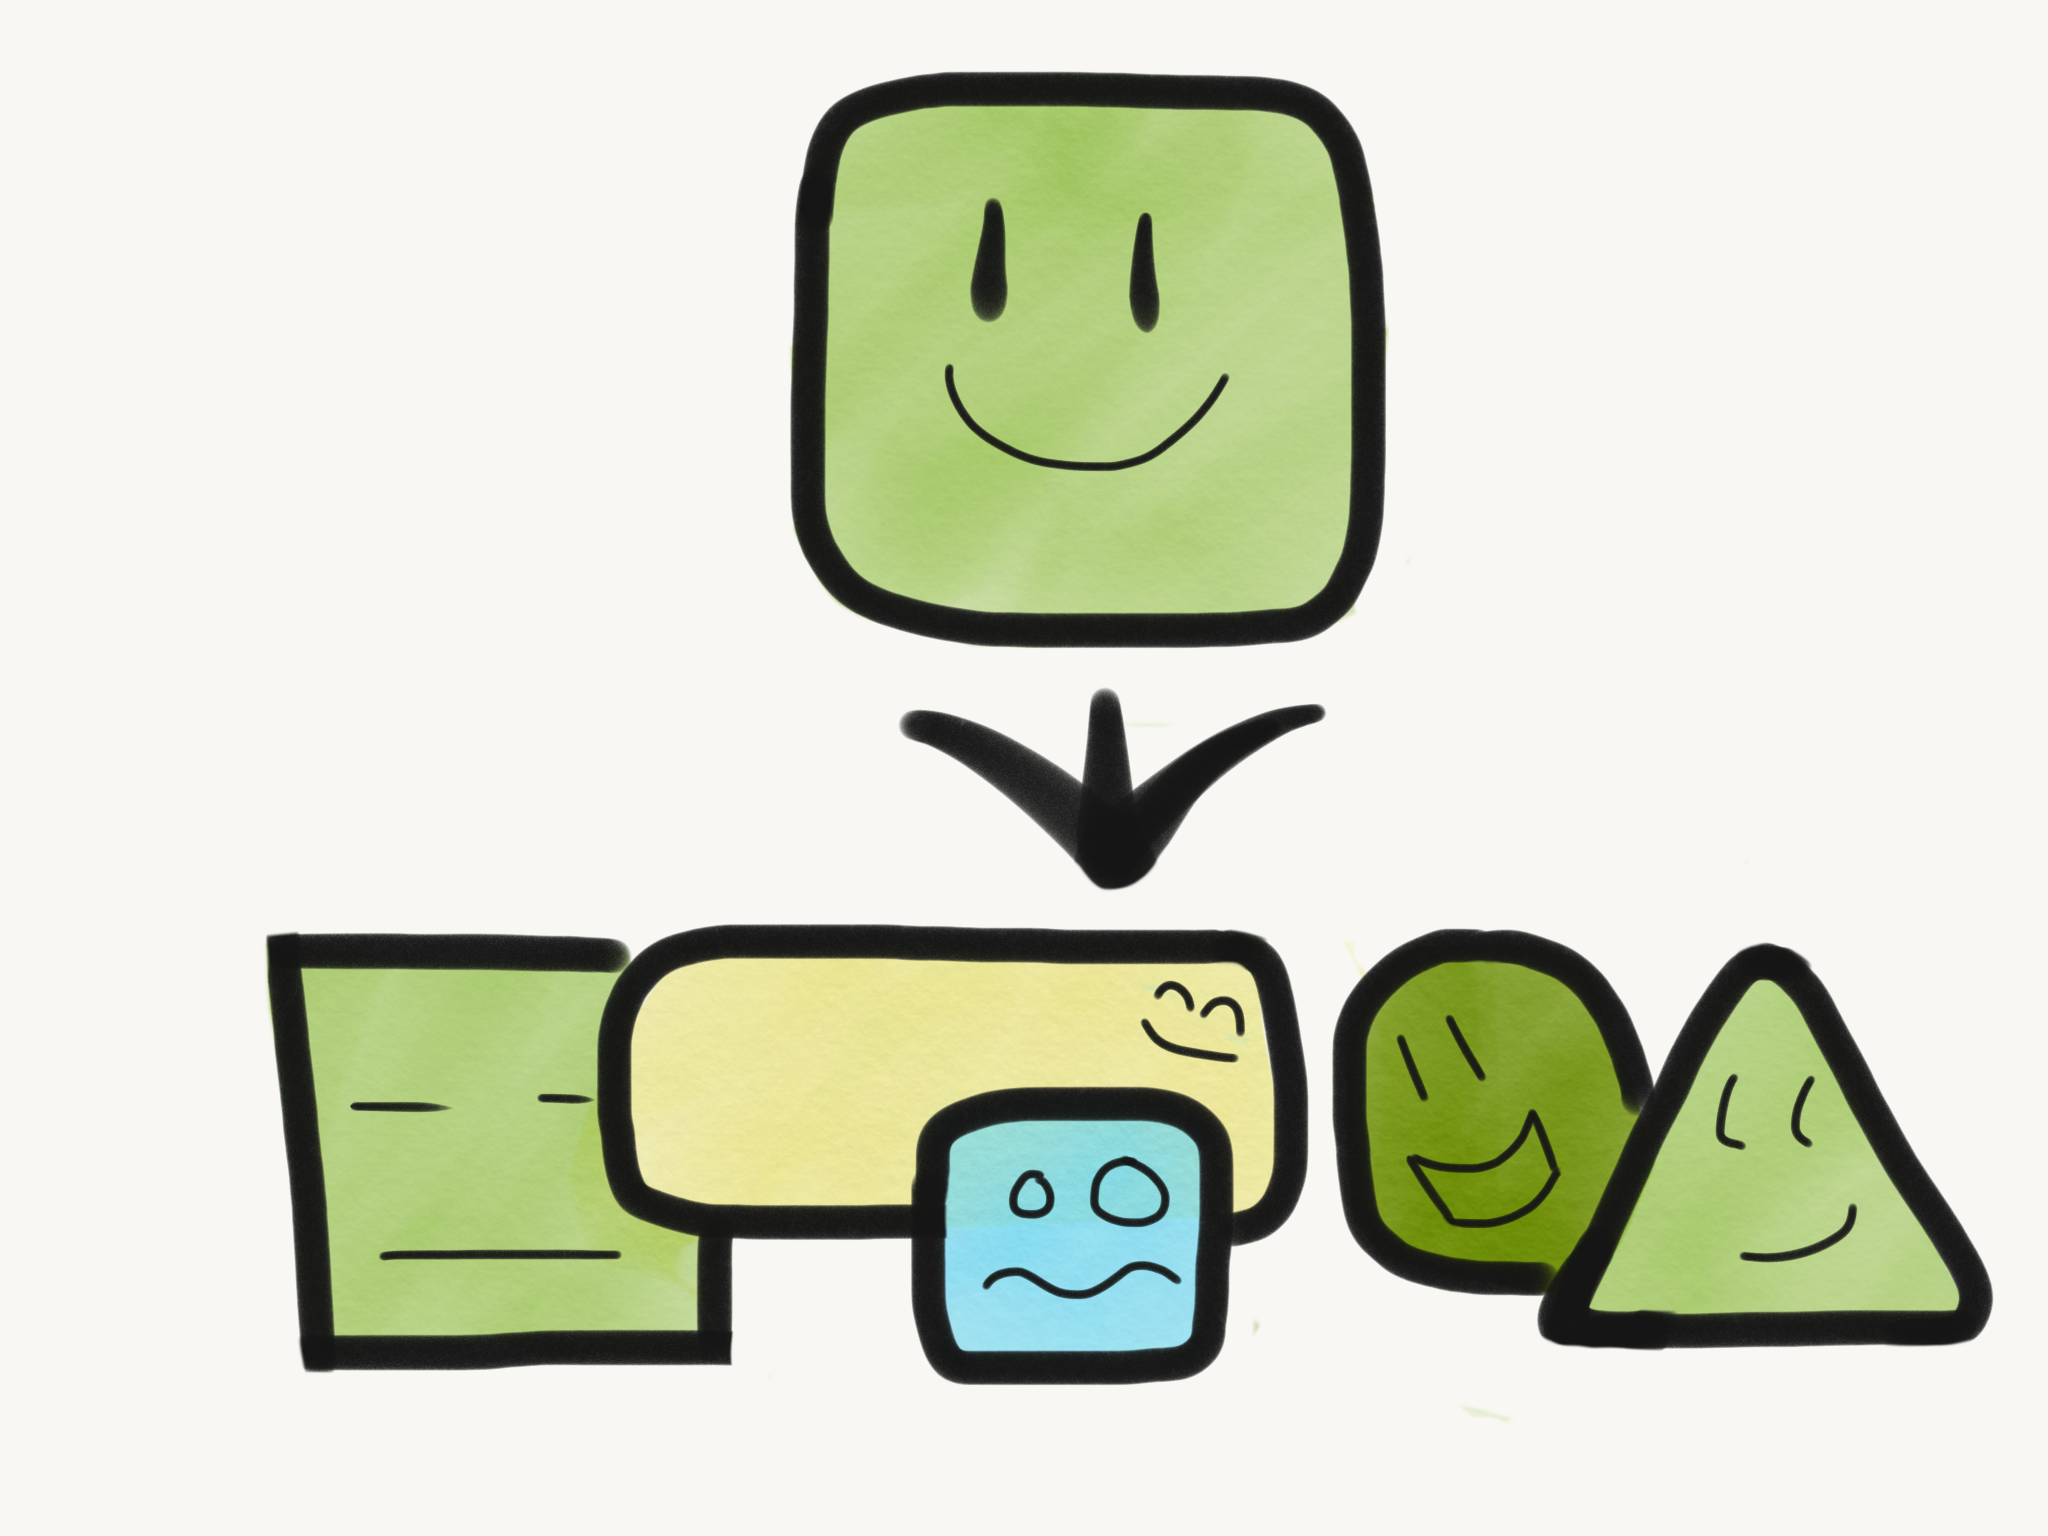
\includegraphics[width=\textwidth]{img/individual_evolvability.png}
        \caption{high individual evolvability}
        \label{subfig:canalization}
    \end{subfigure}%
    \hfill
    \begin{subfigure}[b]{0.5\textwidth}
        \centering
        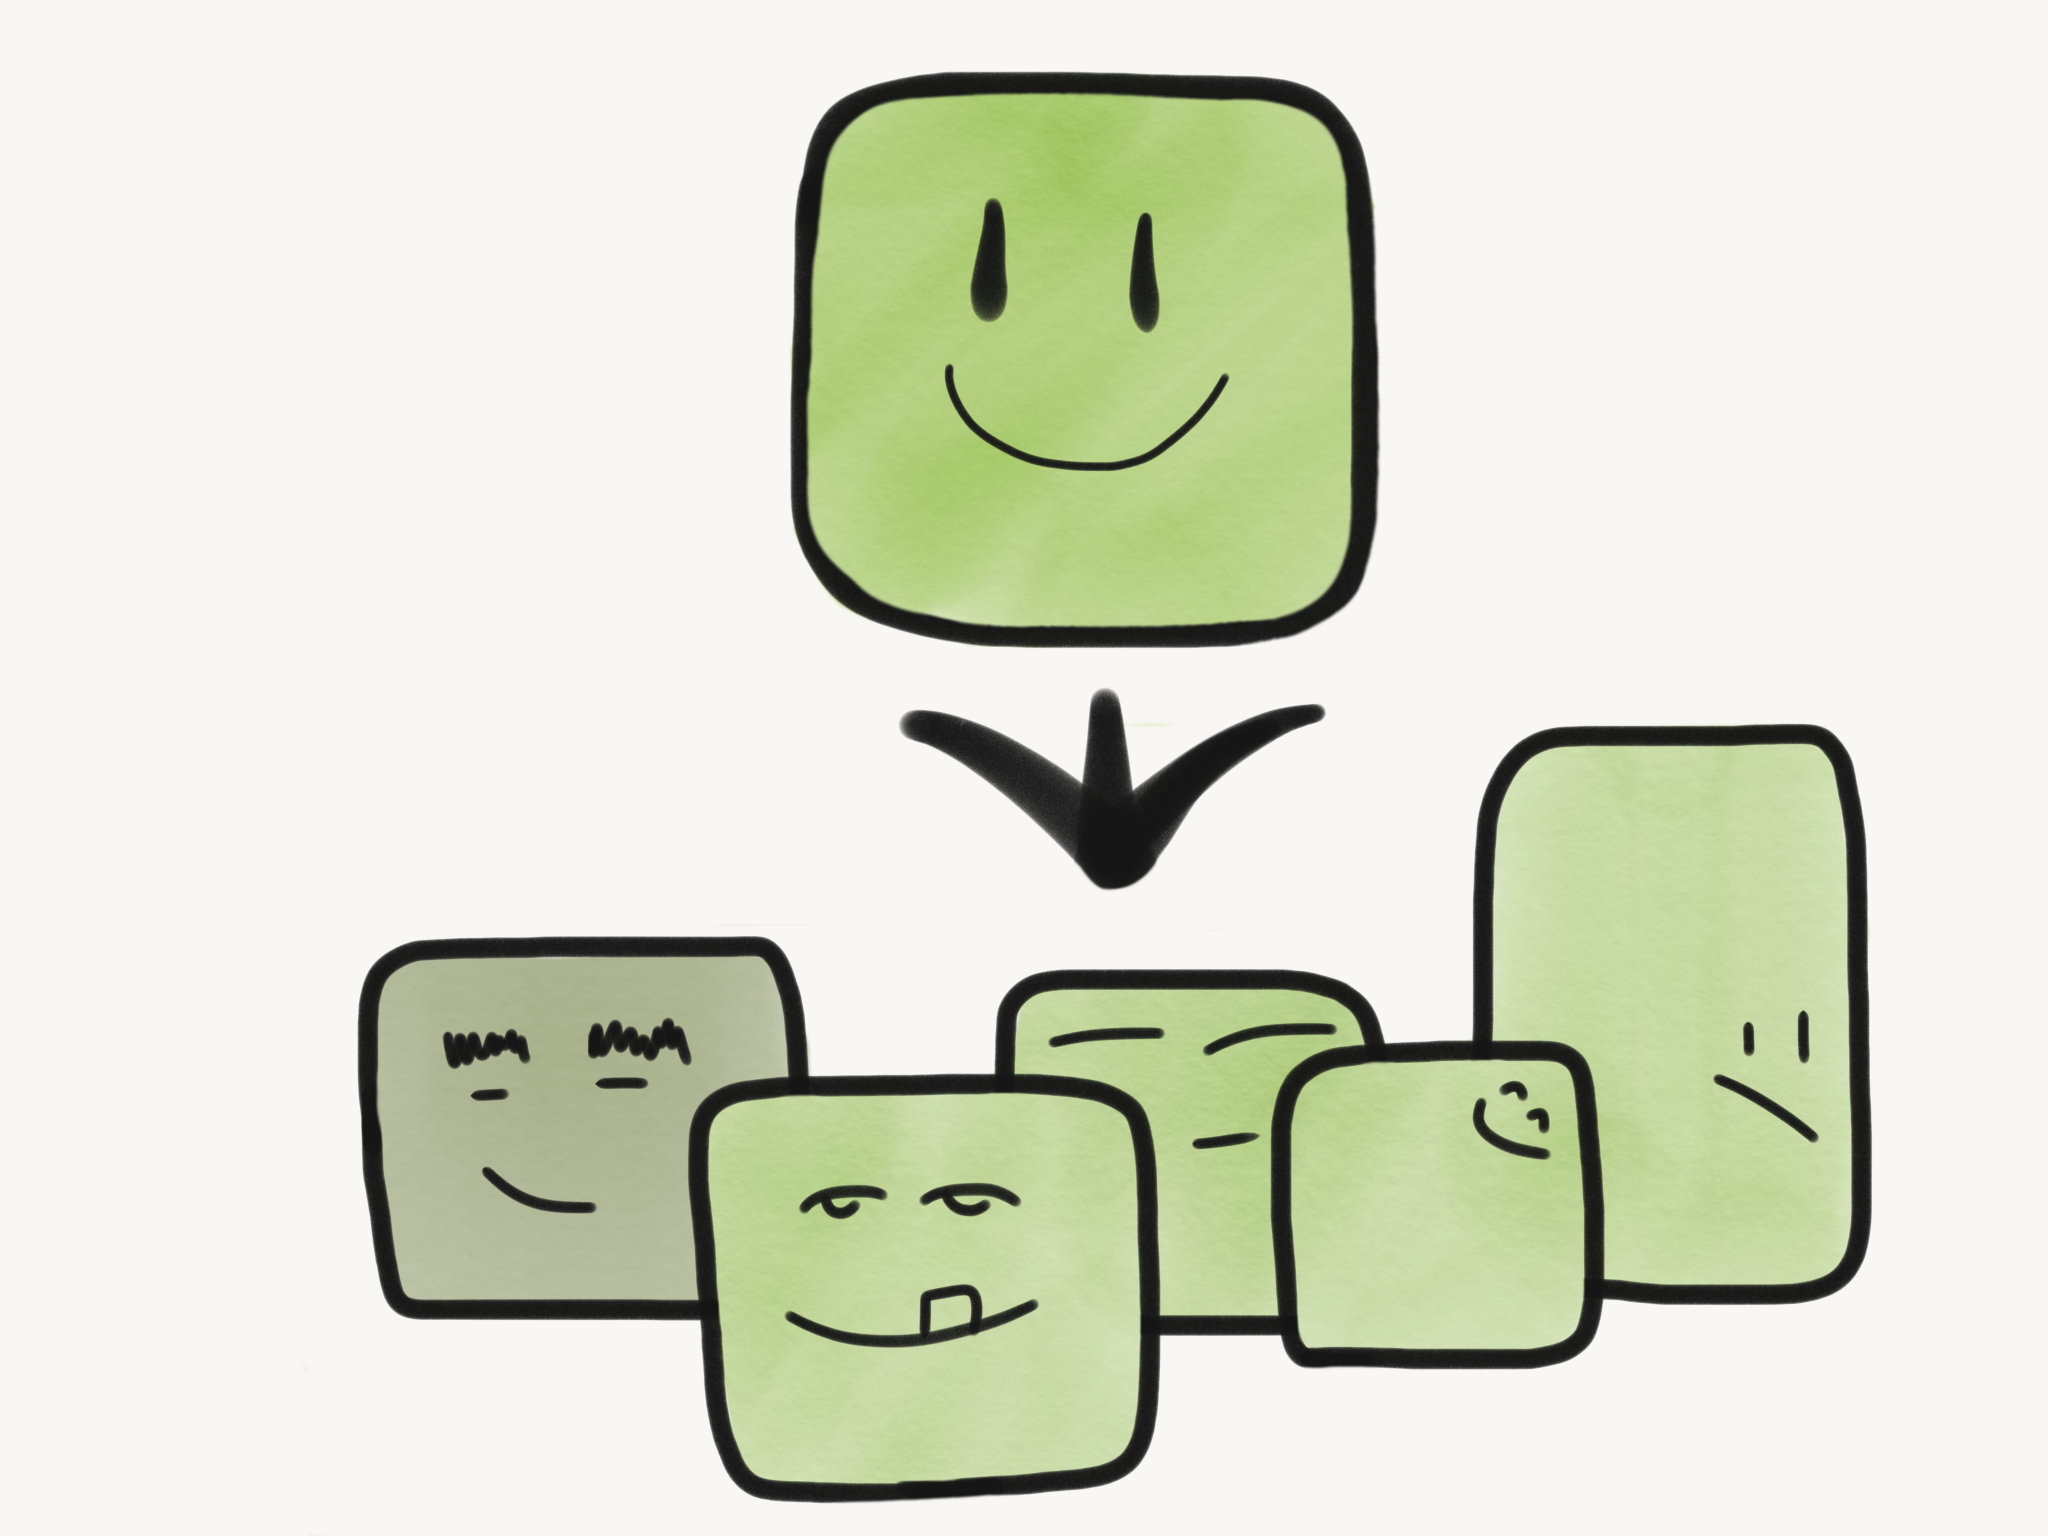
\includegraphics[width=\textwidth]{img/low_individual_evolvability.png}
        \caption{low individual evolvability}
        \label{subfig:no_canalization}
    \end{subfigure}
 	\captionsetup{singlelinecheck=off,justification=raggedright}
    \vspace{-4ex}
  \captionsetup{singlelinecheck=off,justification=raggedright}
  \caption{An illustration of individual evolvability, considering evolvability as heritable variation \cite{Wilder2015ReconcilingEvolvability}.}
  \label{fig:high_vs_low_individual_evolvability}
\end{figure}